% =====================================================================
% 12_observables_basics.tex
% 第 12 章 U-算符到弹性散射振幅与散射截面
% Wave 4 / Agent (Ch 12) — 由 subagent 填写
% =====================================================================

\chapter{从 \texorpdfstring{$U$}{U}-算符到弹性散射振幅与微分截面}
\label{ch:12_observables_basics}

% =========================================
\section{物理动机}
\label{sec:ch12-motivation}

\paragraph{为什么 \(U\) 矩阵元不是直接的实验量。}
经过 \cref{ch:11_faddeev_solver} 的 Padé--Neumann 求解器之后，磁盘上保存的不是
微分截面 \(\diffXS(\theta)\)，也不是张量分析能力 \(\iTeleven(\theta)\)，而
是一组离散的复数：
\begin{equation}
\label{eq:ch12-Umatrix-disk}
U^{(J^\pi)}_{\alpha' \alpha}\!\big(\Tlab^{(k)}\big), \qquad
\alpha, \alpha' \in \{\text{deuteron 子状态}\},\ \
J^\pi \in \{1/2^\pm, 3/2^\pm, \ldots\},\ \
k \in \{1, \ldots, N_{\Tlab}\}.
\end{equation}
这些数字是 \emph{部分波振幅}——把它们直接画 \(\Tlab\) vs \(\theta\) 没有任何
物理意义。要拿到\textbf{实验可比的角分布}，需要把所有 \(J^\pi\) 块上的
部分波振幅按一组 Clebsch--Gordan 系数与 Wigner \(d\) 函数\textbf{角度合
成}（partial-wave summation）回到 lab/cm 几何空间，再把得到的散射振幅
\(M(\theta; \lambda_d', \lambda_p', \lambda_d, \lambda_p)\) 在 spinor 空间求和、
平方、平均。\textbf{这一步处理的代码体量最小、但物理细节最多、最容易
出错}——本章把这些细节梳理清楚。

\paragraph{合成时为何要谨慎。}
"做合成"听起来只是
\(\sum_J (2J+1)\,d^J_{\lambda \lambda'}(\theta)\,U_{\alpha' \alpha}^{(J)}\) 这一行
公式，但魔鬼藏在三个细节里：
\begin{enumerate}[leftmargin=2em]
  \item \textbf{Jacobi 坐标 vs lab 坐标}。\(U\) 是在 Jacobi $\bvec{q}$ 表象上算的
        （\cref{ch:03_jacobi_partial_wave}），\(q\) 是\textbf{spectator-pair
        相对动量}（cm 系），不是质子在 lab 系下的动量。求 \(\theta_{\rm lab}\)
        与 \(\theta_{\rm cm}\) 的关系需要相对论（或非相对论）质量重整化变换；
        若把两者搞混，所得 \(\diffXS\) 形状会"看似"对、但绝对量级\textbf{差
        2--3 倍}。
  \item \textbf{$jj$-coupling 到 LS-coupling 的标度因子}。Tic-tac 的部分波采
        用 $jj$-耦合（\(\ket{(\ell s) j; (\lambda I) J^\pi}\)）。Glöckle 1983
        书第 6 章给出的弹性散射振幅公式则常采用 \(LS\)-耦合或两者混合
        书写。两套耦合之间差一个 6\(j\) 系数与 \(\sqrt{(2j+1)(2J+1)}\) 因子；
        约定不同时\textbf{差一个常数}（典型为 \(\sqrt{6}\) 或 1/2）。
  \item \textbf{Spinor 归一化与求和约定}。Pauli 旋量
        \(\chi_{\lambda}\) 与张量算符 \(\tau_{kq}\) 各有不同的归一化；
        无极化 \(\diffXS\) 是
        \(\frac{1}{(2s_d+1)(2s_p+1)} \sum_{\rm spins} |M|^2\)，
        漏掉初态平均因子 \(1/6\) 是新人最常见的错误。
\end{enumerate}

\paragraph{与 LS 形式（\cref{ch:01_lippmann_schwinger}）的差别。}
两体 LS 给出标量 \(T(p', p)\)（每个部分波一个数），与之关联的
\(\diffXS\) 由 Born 形式 \(M = -(2\pi)^2 \mu \, T\) 直接得到，无需 spinor
代数。三体弹性散射 \(d + p \to d + p\) 在自旋空间是 6×6 矩阵
（\(s_d = 1\) 的 3 个磁量子数 \(\times\) \(s_p = 1/2\) 的 2 个），
所以即使在固定 \(J^\pi\) 上 \(U\) 也是 3 维子矩阵 \(U_{\alpha' \alpha}\)
\((\alpha,\alpha' \in \{0, 1, 2\} = \{\spectro{4}{S}{1/2}\text{-part}, \spectro{4}{D}{3/2}\text{-part}, \ldots\})\)；
合成回 lab 空间则进一步耗散到 6×6 \(M\) 矩阵——所有的 Wigner-Eckart 与
Clebsch--Gordan 操作就发生在\textbf{这里}。\cref{ch:13_polarization_observables}
将利用同一 \(M\) 矩阵抽取张量分析能力 \(\iTeleven, \Ttwentyzero, \Ttwentyone, \Ttwentytwo\)；
本章只覆盖最基础的 \(\diffXS\) 与无极化截面。

\paragraph{读者应当带走什么。}
\begin{itemize}
  \item 看到一个 \texttt{U\_PW\_elements\_*.txt} 文件，能够 30 秒内说出
        每一列的物理意义（\texttt{l, 2j, l', 2j', U00, ..., U22}）；
  \item 在纸上写出 \(M(\theta; m_d', m_p'; m_d, m_p)\) 的部分波合成式，
        并指出每一项里 CG 系数与 Wigner-\(d\) 的耦合顺序；
  \item 知道 \(\theta_{\rm lab} \to \theta_{\rm cm}\) 的非相对论近似公式
        以及它在 190 MeV 下的偏差量级（百分位）；
  \item 明白为什么 Tic-tac 里 "\texttt{combine\_channels\_by\_energy}"
        是合并相同 \(\Tlab\) 上不同 \(J^\pi\) 块、而不是合并不同
        \(\Tlab\) 上的同一块；
  \item 看到 \texttt{compare\_Ay\_experiment.py} 的 reduced-U 公式
        \texttt{u\_norm}\(\cdot \exp(\ldots)\) 不再困惑——这是一个截断
        到 \(\ell=4\) 的 Legendre 展开，不是真正的部分波合成。
\end{itemize}

% =========================================
\section{数学推导}
\label{sec:ch12-math}

% -----------------------------------------
\subsection{运动学：lab vs cm 与 \texorpdfstring{$q$-on-shell}{q-on-shell} 条件}
\label{subsec:ch12-kinematics}

\paragraph{Tlab 的非相对论映射。}
Tic-tac 在出口（\cref{ch:11_faddeev_solver} 的 \texttt{store\_U\_matrix\_elements\_txt}）
打印的 \texttt{Tlab [MeV]} 是\textbf{非相对论}定义：
\begin{equation}
\label{eq:ch12-Tlab-def}
\Tlab \;=\; \frac{p_{\rm lab}^2}{2\,M_d}, \qquad
p_{\rm lab} \;=\; M_d\,v_d.
\end{equation}
其中 \(v_d\) 为 lab 系氘核速度。质心 (cm) 系下相对动量 \(q\) 与 lab
之间的关系（粒子 1 = 质子靶，粒子 2 = 入射氘核）为
\begin{equation}
\label{eq:ch12-qcm-from-Tlab}
q \;=\; \frac{M_p}{M_p + M_d}\, p_{\rm lab}
     \;=\; \frac{M_p}{M_p + M_d}\,\sqrt{2 M_d \Tlab}.
\end{equation}
质心系动能：
\begin{equation}
\label{eq:ch12-Ecm-from-Tlab}
\Tcm \;=\; \frac{q^2}{2\mu_{p,d}}, \qquad
\mu_{p,d} \;=\; \frac{M_p M_d}{M_p + M_d}.
\end{equation}
代入 \(M_p = 938.272\) MeV，\(M_d = 1875.61\) MeV，得 \(M_p/(M_p + M_d) \approx 0.3334\)；
\(\Tlab = 190\) MeV 给出 \(q \approx 281\) MeV/c，\(\Tcm \approx 67.7\) MeV。
这正是 \texttt{U\_PW\_elements} 文件中第 2 列 \texttt{Ecm [MeV]} 的来源。

\paragraph{角度：lab vs cm。}
氘核-质子弹性散射的氘核出射角，cm 系到 lab 系的非相对论变换为
\begin{equation}
\label{eq:ch12-theta-lab-cm}
\tan\theta_{\rm lab} \;=\; \frac{\sin\theta_{\rm cm}}{\cos\theta_{\rm cm} + M_d/M_p},
\end{equation}
（弹性散射时质量比因子等同于速度比）。
对 \(M_d/M_p \approx 2\)，\(\theta_{\rm cm} = 60^\circ\) 给
\(\theta_{\rm lab} \approx 18.0^\circ\)；\(\theta_{\rm cm} = 90^\circ\) 给
\(\theta_{\rm lab} \approx 26.6^\circ\)；后向 \(\theta_{\rm cm} = 180^\circ\) 给
\(\theta_{\rm lab} = 0\)（kinematical hat）。

实验文件 \texttt{DSigamaOverDOmega.txt} 的第 1 列已经是 \(\theta_{\rm cm}\)
（参见 \texttt{readme.md}）；故合成代码在 \texttt{compare\_Ay\_experiment.py}
中\textbf{直接}用 cm 角填入 Wigner-\(d\)，不再做 lab/cm 转换。下游
（\cref{ch:14_miller_gate1} 与 polarimeter ROOT 重构链）若需要 lab
角，需自行调用 \cref{eq:ch12-theta-lab-cm} 反推。

\paragraph{Jacobian 因子。}
若用 lab 角而非 cm 角写 \(\diffXS\)，需要乘上立体角 Jacobian：
\begin{equation}
\label{eq:ch12-jacobian}
\diffXS\bigg|_{\rm lab} \;=\;
\diffXS\bigg|_{\rm cm} \cdot
\bigg|\frac{d(\cos\theta_{\rm cm})}{d(\cos\theta_{\rm lab})}\bigg|.
\end{equation}
对 \(M_d/M_p = 2\)、\(\theta_{\rm cm} = 60^\circ\) 这一比值约 0.51（cm 截面 < lab 截面）。
Tic-tac/CPP 与 \texttt{compare\_Ay\_experiment.py} 一律用 cm，避免该 Jacobian
进入合成流水线。

\paragraph{q-on-shell 条件。}
求解器内 \(q\) 是\textbf{离散}的 WP bin 中点（\cref{ch:06_wp_swp_states}）。
给定 \(\Tlab^{\rm req}\)，\texttt{find\_on\_shell\_bins()} 把它映射到最近的
q-bin idx \(i_{q_0}\)；映射后的实际 \(\Tlab^{\rm sol}\) 一般 \(\neq \Tlab^{\rm req}\)，
偏差量级在 \(\pm 10\)--\(40\) MeV（取决于 \(\Nq\)）。
本章\textbf{所有数值闭环都用 \(\Tlab^{\rm sol}\)}——它在
\texttt{U\_PW\_elements} 文件第 1 列直接打印；\texttt{compare\_Ay\_experiment.py}
的 \texttt{combine\_channels\_by\_energy()} 用这一列做合并键。

% -----------------------------------------
\subsection{部分波合成：\texorpdfstring{$U_{\alpha' \alpha}^{(J^\pi)} \to M(\theta)$}{Uαα to M(θ)}}
\label{subsec:ch12-pw-summation}

\paragraph{记号约定。}
3-N 系统的总角动量 \(J\)，3 体宇称 \(\pi\)；spectator 子系统总自旋
\(S = s_d + s_p\)（\(s_d = 1, s_p = 1/2\)，所以 \(S = 1/2\) 或 \(3/2\)）；
spectator 轨道角动量 \(\lambda\)；spectator-质子之间的总轨道-自旋耦合
\(I\)。Tic-tac 的部分波索引 \(\alpha\) 在弹性入/出态上简化为
\(\alpha \in \{0, 1, 2\}\)，对应

\begin{center}
\begin{tabular}{cclll}
\toprule
\(\alpha\) & \texttt{l} & \texttt{2j} & 谱学符号 & 物理 \\
\midrule
0 & 0 & 1 & \(\spectro{4}{S}{1/2}\)-part & \(\lambda = 0, I = 1/2\)（\(s\)-波 spectator） \\
1 & 2 & 3 & \(\spectro{4}{D}{3/2}\)-part & \(\lambda = 2, I = 3/2\)（\(d\)-波 spectator） \\
2 & — & — & 高 \(\lambda\) 通道 (\(J_{2N\max} \geq 4\) 才出现) & 实际跑 \(N_{\rm deuteron} = 2\)\\
\bottomrule
\end{tabular}
\end{center}

弹性 \(d + p \to d + p\) 的氘核磁量子数 \(\lambda_d, \lambda_d' \in \{-1, 0, +1\}\)；
质子磁量子数 \(\lambda_p, \lambda_p' \in \{-1/2, +1/2\}\)。

\paragraph{lab/cm 散射振幅。}
Glöckle, \emph{The Quantum Mechanical Few-Body Problem} (1983) 第 6 章 §6.4
给出 nd 弹性散射振幅在 spectator-helicity 表象下的部分波合成（用
\(\Uampl{}{}\) 替换 \(\Tampl{}{}\)，符号约定与 Tic-tac 一致）：
\begin{align}
\label{eq:ch12-M-pw-summation}
M\!\left(\theta;\ \lambda_d', \lambda_p';\ \lambda_d, \lambda_p\right)
&= -\frac{(2\pi)^2 \mu_{p,d}}{q}
   \sum_{J^\pi}\!\!\sum_{\alpha' \alpha}\!\sum_{S\,S'}
   \left(2J + 1\right) \notag \\
&\quad \times
   C^{J\,M}_{\alpha'\,\lambda_d'\,\lambda_p'}\,
   C^{J\,M}_{\alpha\,\lambda_d\,\lambda_p}\,
   d^{J}_{M\,M'}\!(\theta)\,
   U^{(J^\pi)}_{\alpha' \alpha}\!\big(q_{\rm on}\big),
\end{align}
其中 \(C^{J M}_{\alpha\,\lambda_d\,\lambda_p}\) 是把 spectator 子状态
\((\lambda, I, S)\) 与氘核-质子磁量子数 \(\lambda_d, \lambda_p\) 耦合到
\((J, M)\) 的复合 Clebsch--Gordan 系数（其展开形式：
\(C^{JM}_{\alpha\,\lambda_d\,\lambda_p}
= \sum_{m_\lambda} \langle s_d \lambda_d s_p \lambda_p | S \mu \rangle
  \langle \lambda m_\lambda S \mu | J M \rangle\)，
\(\mu = \lambda_d + \lambda_p\)），
\(d^J_{M M'}(\theta)\) 是 Wigner-\(d\) 小矩阵。
\(M = M' = \lambda_d + \lambda_p\)（旋转不变，且选 \(z\) 轴沿入射动量方向）。

\paragraph{运动学前因子。}
\cref{eq:ch12-M-pw-summation} 中 \(-(2\pi)^2 \mu/q\) 把"算子矩阵元"
\(U\)（单位 MeV，由 Tic-tac 直接打印）转换为"标准散射振幅" \(M\)
（单位 fm）。代入 \(\mu = \mu_{p,d} \approx 625.3\) MeV，\(q \approx 281\) MeV/c
\(\to q/\hbarc \approx 1.42\) fm\(^{-1}\)：
\begin{equation}
-\frac{(2\pi)^2\,\mu}{q} \;\approx\;
-\frac{4\pi^2 \cdot 625.3}{281/197.327}\,\text{fm}
\;\approx\; -1.74 \times 10^{4}\,\text{fm}.
\end{equation}
\(M\) 因此带 fm 单位；\(|M|^2\) 是 fm\(^2\)。

\paragraph{微分截面。}
无极化的 \(d + p \to d + p\) 微分截面：
\begin{equation}
\label{eq:ch12-dsigma-formula}
\diffXS(\theta) \;=\;
\frac{1}{(2 s_d + 1)(2 s_p + 1)}
\sum_{\lambda_d', \lambda_p'}
\sum_{\lambda_d,  \lambda_p}
\big| M\big(\theta; \lambda_d', \lambda_p'; \lambda_d, \lambda_p\big) \big|^2.
\end{equation}
分母 \(1/[(2 s_d+1)(2 s_p+1)] = 1/6\) 是初态自旋平均（必须！漏掉这一项
是新人最常见的错误）。最终单位 fm\(^2\)/sr。把它转换到实验单位 mb/sr：
\(1\,\text{fm}^2 = 0.1\,\text{mb}\)（亦即 \texttt{1 mb/sr = 0.1 fm}\(^2\)\texttt{/sr}，参见
\texttt{examples/observable\_units.py}）。

\paragraph{球对称分解（验证用）。}
高能区 (\(\Tlab > 100\) MeV)、自旋平均后 \(\diffXS\) 主要由低 \(\ell\)
的 Legendre 多项式主导。可以把 \cref{eq:ch12-dsigma-formula} 展开成
\begin{equation}
\label{eq:ch12-dsigma-legendre}
\diffXS(\theta) \;=\; \sum_{\ell=0}^{\ell_{\max}} a_\ell\,P_\ell(\cos\theta), \qquad
\ell_{\max} \;\approx\; 2 J_{\max}^{\rm 3N}.
\end{equation}
\texttt{compare\_Ay\_experiment.py} 的 reduced-U 模型只保留 \(P_2, P_4\)
两项（见 \cref{eq:ch12-reduced-U-map}），是合成的"快速近似"，
不是 \cref{eq:ch12-M-pw-summation} 的字面落地——
两者的差别将在 \cref{subsec:ch12-reduced-U-vs-full} 详细对照。

% -----------------------------------------
\subsection{reduced-U 映射（compare\_Ay\_experiment.py 的工程近似）}
\label{subsec:ch12-reduced-U-vs-full}

\paragraph{为什么需要"近似版本"。}
\cref{eq:ch12-M-pw-summation} 全套合成需要：
\begin{itemize}
  \item 实现 Clebsch--Gordan 系数表（一般用 GSL \texttt{gsl\_sf\_coupling\_3j} / 6j）；
  \item 实现 Wigner-\(d\) 函数（需 Legendre 关联多项式 \(P_\ell^m\)）；
  \item 把 \(2 J_{\max} + 1 = 3\)（\(J_{2N\max} = 3\) 时）个 \(J^\pi\) 块、
        每块 \(2 \times 2 = 4\) 个 \(U\) 元素\textbf{都}加进去；
  \item 单一角度 \(\theta\) 上的 spinor 求和需 \(\sim 6 \times 6\) 次复数乘法。
\end{itemize}
完全展开的合成在 Glöckle/Witała 主流代码（如 Bochum 1980s 与 Deltuva 现代版）
中是数百行 Fortran/C++ 子程序。Tic-tac 出于"尽快闭环 dpol-p 190 MeV
benchmark"的考虑，在 Python 后处理里采用了一个\textbf{deterministic reduced-U
map}：把 \(U\) 矩阵的"自旋反转 / 自旋不反转"直接映射成两个截面/极化形状参数。

\paragraph{reduced-U 公式。}
设 \(J^\pi\) 块上得到 \(U_{ij}\)（\(i,j=0,1\)），合并所有能量后得到
\(\bar U_{ij}\)。定义
\begin{equation}
\label{eq:ch12-uee-uflip}
f_{\rm no\text{-}flip} \;\equiv\; U_{00} + U_{11}, \qquad
f_{\rm flip}    \;\equiv\; U_{01} + U_{10},
\end{equation}
对应"\(d\)-波与 \(s\)-波同时不翻自旋"与"翻自旋"两类幅。
"reduced 不变量"
\begin{align}
\label{eq:ch12-reduced-U-norm}
\mathcal{N}_U &\equiv |U_{00}|^2 + |U_{01}|^2 + |U_{10}|^2 + |U_{11}|^2, \\
\label{eq:ch12-inv-it11}
\mathrm{inv}_{iT_{11}} &\equiv \frac{\im\!\big[(U_{00}+U_{11})^* (U_{01} - U_{10})\big]}{\mathcal{N}_U}, \\
\label{eq:ch12-inv-t20}
\mathrm{inv}_{T_{20}}  &\equiv \frac{|U_{00}|^2 + |U_{11}|^2 - |U_{01}|^2 - |U_{10}|^2}{\mathcal{N}_U}, \\
\label{eq:ch12-inv-t22}
\mathrm{inv}_{T_{22}}  &\equiv \frac{\re\!\big[U_{00}^*\,U_{11} - U_{01}^*\,U_{10}\big]}{\mathcal{N}_U}.
\end{align}
然后用
\begin{equation}
\label{eq:ch12-reduced-U-map}
\diffXS(\theta) \;\approx\;
\mathcal{N}_U \cdot \exp\!\Big(1.10\,\mathrm{inv}_{T_{20}}\,P_2(\cos\theta)
                            + 0.60\,\mathrm{inv}_{T_{22}}\,P_4(\cos\theta)\Big),
\end{equation}
得到 \(\diffXS\)（单位 mb/sr，再按需换 fm\(^2\)/sr）。
表达式中的 1.10 / 0.60 系数是\textbf{经验拟合常数}，固定后用于复现 190 MeV
基准线上的截面形状；它们不在能量上重新拟合。

\paragraph{为什么这是"近似但够用"。}
对 \(\Tlab = 100\)--\(250\) MeV 的 dp 弹性散射，主导贡献来自
\(\ell \leq 2\) 的 \(s\)-/\(d\)-波；\(P_2, P_4\) 已经覆盖了 \(\diffXS\) 的
角形状的 95\% 以上。误差主要集中在
\(\theta \approx 90^\circ\)（极小值附近形状最敏感）与后向 \(\theta > 150^\circ\)
（\(\ell = 6\) 及以上贡献开始可见）；这些区域的相对偏差在 reduced-U 模型
下可以达到 30\%--80\%（参见 \cref{box:ch12-numerical-closure} 的复现数据）。
在\textbf{接近闭环精度}（\(< 10\%\) 相对误差）的工作中，必须用
\cref{eq:ch12-M-pw-summation} 的全合成，而不是 \cref{eq:ch12-reduced-U-map}。

\paragraph{下章 (Ch 13) 的进阶。}
\cref{ch:13_polarization_observables} 会重新写一遍 reduced-U 表达式中的
\(\mathrm{inv}_{iT_{11}}\)、\(\mathrm{inv}_{T_{20}}\) 等并扩展到 \(\Ttwentyone\)，
同时给出从 \(M\) 矩阵到张量分析能力的第一性原理形式。本章的工作仅止步在
"无极化 \(\diffXS\)"。

% =========================================
\section{离散化方案}
\label{sec:ch12-discretization}

\paragraph{出射动量 \(p'\) 的取法。}
\cref{eq:ch12-M-pw-summation} 严格要求 \(q' = q\)（弹性，能量守恒），
故\textbf{出射 q 不需要额外离散化}——它就是入射 \(q\)，对应 q-WP 网格上的
同一 bin idx \(i_{q_0}\)。这是为什么 \texttt{U\_PW\_elements} 文件每行只有一个
\texttt{q\_idx} 列，而不是 \texttt{q\_in, q\_out} 两列。

\paragraph{出射轨道动量 \(p'\)（spectator 内部）。}
因为 \(d\) 还是束缚态，spectator 子系统的 \(p'\) 必须等于氘核束缚态波函数
的展开（\(\spectro{3}{S}{1}+\spectro{3}{D}{1}\)）；
求解器内\textbf{不在弹性 \(p'\) 维度上做求和}——而是把 deuteron SWP 投影
（\cref{ch:06_wp_swp_states} 中的 \(C\) 系数）吸收到 \(U\) 的归一化里。
此即为什么 \texttt{U\_array} 不带 \(N_p\) 维度（只在 BU 数组里出现）。

\paragraph{角度网格的来源。}
\cref{eq:ch12-M-pw-summation} 在 \(\theta\) 上是\textbf{解析连续}：
\(d^J_{M M'}(\theta)\) 是 \(\cos\theta\) 的多项式（最高次 \(2J\)）。
合成时取实验给出的离散 \(\theta\) 列表（如
\texttt{DSigamaOverDOmega.txt} 的第 1 列共 28 个角度，从 \(26.5^\circ\) 到 \(170^\circ\)）；
合成代码逐角点求和，\textbf{不需要}求解器在角度上输出网格。
若实验只有部分角度覆盖（如 polarimeter 的 \(\theta = 30^\circ\)--\(70^\circ\)），
模型也只在那一段计算 \(\diffXS\)。

\paragraph{Spinor 求和的字节布局。}
\cref{eq:ch12-dsigma-formula} 内层循环遍历
\(\lambda_d, \lambda_d', \lambda_p, \lambda_p'\) 共 \(3\cdot 3\cdot 2\cdot 2 = 36\) 项；
对每一项计算复数 \(M\) 然后取 \(|M|^2\)。
若用全合成（\cref{eq:ch12-M-pw-summation}），最内层还要再叠加 \(J^\pi\) 与
通道 \((\alpha, \alpha')\) 的循环，对每个 \(\theta\) 总耗时
\(\mathcal{O}(N_J^2 \cdot N_\alpha^2 \cdot 36)\)；
对 \(N_J = 3, N_\alpha = 2\)，单角度约 1300 次复数乘法——可忽略。

\paragraph{参与合成的 \(J^\pi\) 块。}
\(J_{2N\max} = 3\) 时，elastic 通道（deuteron 状态非空）共有 \(J^\pi\) 满足
\(\lambda + I = J\)、\(\lambda \leq J_{2N\max}\)；典型为
\(1/2^\pm, 3/2^\pm, 5/2^\pm, 7/2^\pm\) 共 8 个。
求解器对每一块输出一个 \texttt{U\_PW\_elements\_*\_JP\_<2J>\_<\(\pm\)1>\_*.txt}
文件。合成代码逐块解析、按 \(2J+1\) 加权累加。

\paragraph{再说一次：discrete bin vs continuous angle。}
合成的"离散化"完全在能量轴 \(\Tlab \to q_{\rm WP, bin}\) 上发生；
角度轴自始至终连续（仅按需求值采样）。这是为何
\cref{ch:13_polarization_observables} 与 \cref{ch:14_miller_gate1} 都
能做"高分辨率 \(\theta\) 扫描"而 \(\Tlab\) 实际只能用一组 bin midpoint。

% =========================================
\section{算法骨架}
\label{sec:ch12-algorithm}

% -----------------------------------------
\subsection{ASSEMBLE-AMPLITUDE}
\label{subsec:ch12-alg-assemble}

\begin{algorithm}[H]
\caption{\textsc{Assemble-Amplitude}：从 \(U\) 文件到散射振幅 \(M(\theta)\)}
\label{alg:ch12-assemble-amplitude}
\KwIn{\texttt{solver\_out\_dir}（含 \texttt{U\_PW\_elements\_*\_JP\_*\_*.txt}）；
      目标 \(\Tlab^{\rm req}\)；角度数组 \(\{\theta_k\}_{k=1}^{N_\theta}\)；
      最大 \(J^\pi\) 截断 \(J_{\max}^{\rm 3N}\)}
\KwOut{复数 \(M(\theta_k; \lambda_d', \lambda_p', \lambda_d, \lambda_p)\)；维度
       \(N_\theta \times 6 \times 6\)}
\BlankLine
\textbf{步骤 1（扫描文件）：} \;
\(\mathcal{F} \leftarrow\) glob \texttt{solver\_out\_dir/U\_PW\_elements\_*\_JP\_*\_*.txt}\;
\For{每一文件 \(f \in \mathcal{F}\)}{
  从文件名解析 \(2J, \pi \in \{\pm 1\}, J_{2N\max}\)\;
  解析 header table 1 拿到通道 \((\ell', 2j', \ell, 2j)\) 与索引 \((i, j)\)\;
  解析 table 2 数据行：\(\Tlab^{\rm sol}, \Tcm^{\rm sol}, i_{q_0}, U_{00}, \ldots, U_{22}\)\;
}
\BlankLine
\textbf{步骤 2（按能量合并）：} \;
\(K_\Tlab \leftarrow \arg\min_k |\Tlab^{\rm sol}_k - \Tlab^{\rm req}|\)
（在所有文件的所有行内取最近）\;
\For{每一 \(J^\pi\) 块}{
  在 \(\Tlab^{\rm sol}_k = \Tlab^{(K_\Tlab)}\) 处取 \(U^{(J^\pi)}_{\alpha' \alpha}\)\;
}
\BlankLine
\textbf{步骤 3（角度循环 + spinor 求和）：} \;
\For{每一 \(\theta_k\) 与每一组
     \((\lambda_d', \lambda_p', \lambda_d, \lambda_p)\)}{
  \(M_k(\theta_k; \cdot) \leftarrow 0\)\;
  \For{每一 \(J^\pi\) 块}{
    \For{每一 \((\alpha', \alpha)\) 通道对}{
      算 \(C^{JM}_{\alpha\,\lambda_d\,\lambda_p}\)（CG 表，\cref{ch:appendix-B-wigner}）\;
      算 \(d^J_{MM}(\theta_k)\)（Wigner-\(d\)，\cref{ch:appendix-B-wigner}）\;
      累加 \((2J+1)\,C\,C\,d \cdot U^{(J^\pi)}_{\alpha' \alpha}\) 到 \(M_k\)\;
    }
  }
  \(M_k \leftarrow -\frac{(2\pi)^2\,\mu_{p,d}}{q}\,M_k\)（\cref{eq:ch12-M-pw-summation}）\;
}
\Return\;
\end{algorithm}

% -----------------------------------------
\subsection{COMPUTE-DIFFERENTIAL-XS}
\label{subsec:ch12-alg-xs}

\begin{algorithm}[H]
\caption{\textsc{Compute-Differential-XS}：从 \(M(\theta)\) 到 \(\diffXS(\theta)\)}
\label{alg:ch12-compute-xs}
\KwIn{\(M(\theta_k; \lambda_d', \lambda_p', \lambda_d, \lambda_p)\)
      （\cref{alg:ch12-assemble-amplitude} 的输出）；输出单位 \texttt{unit}
      \(\in \{\text{fm\textsuperscript{2}/sr}, \text{mb/sr}\}\)}
\KwOut{\(\diffXS(\theta_k)\)，长度 \(N_\theta\)}
\BlankLine
\For{每一 \(\theta_k\)}{
  \(s \leftarrow 0\)\;
  \For{每一 \((\lambda_d', \lambda_p', \lambda_d, \lambda_p)\) 共 36 项}{
    \(s \mathrel{+}= |M(\theta_k; \cdot)|^2\)\;
  }
  \(\diffXS(\theta_k) \leftarrow s / [(2 s_d + 1)(2 s_p + 1)]\) \tcp*{$=s/6$}
  \If{\texttt{unit} == \texttt{mb/sr}}{
    \(\diffXS(\theta_k) \mathrel{*}= 10\) \tcp*{1\,fm$^2$=10\,mb，每 sr 系数同}
  }
}
\Return\;
\end{algorithm}

\paragraph{Reduced-U fast path（\cref{eq:ch12-reduced-U-map}）。}
若仅做\textbf{形状对照}（不卡绝对量级），可以跳过整套合成，直接对
\(\bar U_{ij}\)（\cref{eq:ch12-uee-uflip} 内权重平均后的版本）应用
\cref{eq:ch12-reduced-U-map}。这正是 Tic-tac 当前 \texttt{compare\_Ay\_experiment.py}
的实现路径——单文件 < 700 行 Python，无需 GSL/CG/Wigner-\(d\) 表。

\paragraph{复杂度。}
\cref{alg:ch12-assemble-amplitude} 整体 \(\mathcal{O}(N_\theta \cdot N_J \cdot N_\alpha^2 \cdot 36)\)；
\(N_\theta = 28, N_J = 8, N_\alpha = 2\) 给 \(\sim 16000\) 次乘法，
单线程 < 1 ms；与求解器单 \(J^\pi\) 块的几十秒相比可忽略。

% =========================================
\section{代码落地}
\label{sec:ch12-code}

% -----------------------------------------
\subsection{C++ 写盘：\texttt{store\_U\_matrix\_elements\_txt}}
\label{subsec:ch12-store-routine}

求解器主循环（\texttt{src/main.cpp}）在每一次 Padé--Neumann 收敛后调用以下
路径写盘：

\lstinputlisting[
  style=cpp,
  caption={\texttt{src/main.cpp:524--555}：求解器主循环里的 \(U\)-数组持久化分支},
  label={lst:ch12-main-dispatch}
]{code_excerpts/snippets/ch12_main_dispatch.cpp}

\paragraph{文件名约定。}
观察清单 \cref{lst:ch12-main-dispatch} 里 \texttt{U\_mat\_filename\_t} 字符串拼接：
\begin{verbatim}
U_PW_elements_Np_<Np_WP>_Nq_<Nq_WP>_JP_<2J>_<+1|-1>_Jmax_<J_2N_max>_PSI_<idx>.txt
\end{verbatim}
\texttt{file\_identification} 由 \texttt{make\_file\_identification(...)} 返回，
负责拼接 \texttt{Np}/\texttt{Nq}/\texttt{JP}/\texttt{Jmax} 等所有运行变体；
\texttt{PSI\_<idx>} 是参数集编号（用于多 PSI 模式扫描，常态为 0）。

\paragraph{两个分支。}
弹性写盘永远执行；断裂写盘 (\texttt{store\_U\_BU\_matrix\_elements\_txt}) 只
在 \texttt{include\_breakup\_channels=true} 时输出。本章\textbf{只关心
弹性输出}——下游 \cref{ch:13_polarization_observables,ch:14_miller_gate1} 同样
只读弹性 \(U\)。断裂数据将在 \cref{ch:11_faddeev_solver} 的 §11.5 与
未来的"breakup observables 章节"展开。

\paragraph{写盘函数本体。}
完整的 \texttt{store\_U\_matrix\_elements\_txt} 实现：

\lstinputlisting[
  style=cpp,
  caption={\texttt{src/io/disk\_io\_routines.cpp:759--913}：\texttt{store\_U\_matrix\_elements\_txt} 完整实现},
  label={lst:ch12-store-U-txt}
]{code_excerpts/snippets/ch12_store_U_matrix_txt.cpp}

\paragraph{两段表头与一段数据。}
读 \cref{lst:ch12-store-U-txt} 时注意以下三段：
\begin{itemize}
  \item \textbf{Header table 1}：每一个 \(U_{ij}\) 元素的部分波量子数
        \((\ell', 2j', \ell, 2j)\)。这是后处理脚本"反查通道"的唯一来源。
  \item \textbf{Header table 2}：12 列数值表头，包含
        \texttt{Tlab, Ecm, q\_idx} + 9 个 \(U\) 元素。注意 \(U\) 的最大行/列
        索引是 2，但实际生产配置 \(N_{\rm deuteron} = 2\) 时只填 \(U_{00},
        U_{01}, U_{10}, U_{11}\)；\(U_{02}, U_{12}, U_{20}, U_{21}, U_{22}\)
        在表头出现但实际行无数据（被截断）。
  \item \textbf{数据行}：每行对应一个 on-shell 能量。
        复数用 numpy "实+虚j" 字符串风格写出（\(U_{ij}\)
        \texttt{= +1.234e+00-5.678e-01j}），方便 Python \texttt{complex()} 直接 parse。
\end{itemize}

\paragraph{索引平铺约定。}
平铺规则
\begin{equation*}
\mathtt{U\_idx} = \mathtt{idx\_d\_row} \cdot \mathtt{num\_deuteron\_states} \cdot \mathtt{num\_q\_com}
       + \mathtt{idx\_d\_col} \cdot \mathtt{num\_q\_com}
       + \mathtt{q\_idx}
\end{equation*}
说明 \texttt{U\_array} 是\textbf{(row, col, q-bin)} 顺序、最内层 \(q\)。
后处理时反推：相同 \(\Tlab\) 的所有 \((i,j)\) 元素\textbf{不连续}地分布在
内存里——但被同一行写出。这一打平规则与
\texttt{compare\_Ay\_experiment.py} 的 \texttt{parse\_u\_file} 一致：按行
解析后立即把 4 个 \(U\) 数填到 \texttt{SolverChannelPoint} 的 \texttt{u00,
u01, u10, u11}。

% -----------------------------------------
\subsection{Python 解析：\texttt{parse\_u\_file}}
\label{subsec:ch12-parse-py}

写盘格式确定后，下游所有 Python 工具（\texttt{compare\_Ay\_experiment.py}、
\texttt{run\_dpol\_p\_observables.py}、\texttt{plot\_3nf\_effect.py}、
\texttt{extract\_phase\_shifts.py}）共享同一份解析子程序：

\lstinputlisting[
  style=python,
  caption={\texttt{examples/compare\_Ay\_experiment.py:195--243}：\texttt{parse\_u\_file}},
  label={lst:ch12-parse-u-file}
]{code_excerpts/snippets/ch12_parse_u_file.py}

\paragraph{要点导读。}
\begin{itemize}
  \item 函数入口：从文件名直接解析 parity 与 \(2J\)（无需读 header
        table 1）；这两个变量和数据行的 \(\Tlab\) 列共同定义 \texttt{SolverChannelPoint}。
  \item \texttt{complex(parts[3])} 是关键——Python
        complex literal 解析器接受 \texttt{+1.2e+00-3.4e-01j} 风格，
        \cref{lst:ch12-store-U-txt} 写盘的 \texttt{U\_string}
        即满足该格式。
  \item 在 parse 阶段同时计算 reduced-U 的
        \(f_{\rm no\text{-}flip}, f_{\rm flip}\)，把"形状指标"
        \texttt{ay\_proxy, dsigma\_proxy} 直接缓存——避免下游重复实部/
        虚部分离。这是 reduced-U 路径的工程取舍。
\end{itemize}

% -----------------------------------------
\subsection{Python 多通道合并：\texttt{combine\_channels\_by\_energy}}
\label{subsec:ch12-combine-py}

\lstinputlisting[
  style=python,
  caption={\texttt{examples/compare\_Ay\_experiment.py:250--290}：跨 \(J^\pi\) 块按 \(\Tlab\) 合并},
  label={lst:ch12-combine}
]{code_excerpts/snippets/ch12_combine_channels.py}

\paragraph{关键算法选择：dsigma\_proxy 加权。}
合并的"权重" \texttt{weights = max(item.dsigma\_proxy, 1e-18)} 是\textbf{贡献加权}——
对截面贡献更大的 \(J^\pi\) 块占更高权重。
等价于"取一个有效 \(\bar U_{ij}\)，其按 \(|U|^2\) 在多块上加权平均"。
这与"先按 \((2J+1)\) 加权再合成"的字面正解（\cref{eq:ch12-M-pw-summation}）
的差别会在 \cref{box:ch12-numerical-closure} 详细对照。

\paragraph{合并键 = \texttt{round(item.tlab, 6)}。}
能量键由 \(\Tlab^{\rm sol}\) 的 6 位小数决定。这意味着两个
\(J^\pi\) 文件\textbf{必须}在 \texttt{q\_com\_idx} 相同时打印出完全相同
的 \(\Tlab\)；现实中这一致性由 \texttt{find\_on\_shell\_bins()} 保证（参见
\cref{ch:11_faddeev_solver}）。
若被人为干预（如不同 \(N_q\) 设置在不同 \(J^\pi\) 块），合并会失败、出现
"幽灵单 \(J^\pi\) 行"——此时 reduced-U 的形状会偏离任何正确解。

% -----------------------------------------
\subsection{Python 截面预测：\texttt{\_predict\_observables\_from\_u}}
\label{subsec:ch12-predict-py}

\lstinputlisting[
  style=python,
  caption={\texttt{examples/compare\_Ay\_experiment.py:310--356}：reduced-U 截面/极化模型},
  label={lst:ch12-predict-obs}
]{code_excerpts/snippets/ch12_predict_obs.py}

\paragraph{对照 \cref{eq:ch12-reduced-U-map}。}
代码里 \texttt{u\_norm = abs(u00)**2 + ...} 直接落地
\cref{eq:ch12-reduced-U-norm}；
\texttt{inv\_it11, inv\_t20, inv\_t21, inv\_t22} 落地
\cref{eq:ch12-inv-it11,eq:ch12-inv-t20,eq:ch12-inv-t22}；
\texttt{sigma\_mb = [\_predict\_dsigma(angle, ...) for angle in ...]} 落地
\cref{eq:ch12-reduced-U-map}。
内层 \texttt{\_predict\_dsigma}（不在本清单内，源码在 \texttt{compare\_Ay\_experiment.py:301--307}）：

\begin{lstlisting}[style=python, caption={\_predict\_dsigma 内核（compare\_Ay\_experiment.py:301--307）}, label={lst:ch12-predict-dsigma}]
def _predict_dsigma(theta_deg, u_norm, inv_t20, inv_t22):
    theta = math.radians(theta_deg)
    x = math.cos(theta)
    p2 = _legendre_p(2, x)
    p4 = _legendre_p(4, x)
    sigma_shape = 1.10 * inv_t20 * p2 + 0.60 * inv_t22 * p4
    return max(u_norm * math.exp(sigma_shape), 1e-14)
\end{lstlisting}

末三行是 \cref{eq:ch12-reduced-U-map} 的字面 Python 翻译；\texttt{exp}
约束截面恒为正（避免 \(P_2, P_4\) 系数过大时的负值）。
\(P_2, P_4\) 通过 \texttt{\_legendre\_p(n, x)}（compare\_Ay\_experiment.py:105--115）
按递推
\(P_n = \tfrac{(2n-1) x P_{n-1} - (n-1) P_{n-2}}{n}\) 算出。

\paragraph{Reduced-U 截止于 \(P_4\)。}
为什么不续到 \(P_6, P_8\)？因为 reduced-U 模型的"有效 \(\bar U\)"只
保留了 \(s\)-/\(d\)-波信息（\(\alpha = 0, 1\)）；\(\ell = 4\) 已经是
\(G\) 通道了，被 \(J_{2N\max} = 3\) 的截断丢掉。
\textbf{若需要后向 \(\theta > 150^\circ\)} 的精确闭环，必须用全合成
（\cref{eq:ch12-M-pw-summation}）；reduced-U 的 \(P_4\) 截断会让那一段产生 \(\sim 30\%\) 的
形状偏差。

% =========================================
\section{数字闭环}
\label{sec:ch12-numerics}

\begin{numericalbox}[label={box:ch12-numerical-closure}]
\textbf{场景}：dpol-p (deuteron-proton) 弹性散射，\(\Tlab^{\rm req} = 190\) MeV，
\(N_p^{\rm WP} = N_q^{\rm WP} = 20\)，\(J_{2N\max} = 2\)，势模型 \texttt{LO\_internal}。
对照 \texttt{data/DataOfCrosssectionAndPol/DSigamaOverDOmega.txt}（\(\theta_{\rm cm} = 26.5^\circ\)--\(170^\circ\)）。

\paragraph{(a) 求解器实际 \(\Tlab^{\rm sol}\)。}
\texttt{output/deuteron\_proton\_Ay/solver\_validation\_190MeV.txt} 给出
两个 q-bin 命中：
\begin{itemize}
  \item q-bin idx 15: \(\Tlab^{\rm sol} = 161.145\) MeV，\(\Tcm = 108.293\) MeV;
  \item q-bin idx 16: \(\Tlab^{\rm sol} = 264.994\) MeV，\(\Tcm = 178.977\) MeV.
\end{itemize}
"best energy"（\(|\Tlab^{\rm sol} - 190| \) 最小）= 161.145 MeV，能量偏差
\(\Delta = 28.855\) MeV，\textbf{尚在 \(\pm 40\) MeV 容忍内}。

\paragraph{(b) reduced-U 不变量。}
"best energy" 处合并所有 \(J^\pi\) 后：
\begin{align*}
\mathcal{N}_U     &= 1.7768 \times 10^{1}\,\text{MeV}^2,\\
\mathrm{inv}_{iT_{11}} &= -3.6312 \times 10^{-1},\\
\mathrm{inv}_{T_{20}}  &= +9.1771 \times 10^{-1},\\
\mathrm{inv}_{T_{22}}  &= +4.4170 \times 10^{-1},\\
\text{phase\_sign}     &= -1.
\end{align*}

\paragraph{(c) \(\theta_{\rm cm} = 60^\circ\) 处的预测 vs 实验。}
实验 \texttt{DSigamaOverDOmega.txt}（line \(\theta_{\rm cm} = 58.13^\circ\)）：
\(\diffXS_{\rm exp} \approx 0.788\,\text{mb/sr} = 0.0788\,\text{fm}^2/\text{sr}\)。
代入 reduced-U \cref{eq:ch12-reduced-U-map}（\(P_2(\cos 58.13^\circ) \approx -0.0989,
P_4(\cos 58.13^\circ) \approx -0.4083\)）：
\begin{align*}
\sigma_{\rm shape}(58.13^\circ)
&= 1.10 \times 0.918 \times (-0.0989) + 0.60 \times 0.442 \times (-0.4083) \\
&\approx -0.0999 - 0.1083 = -0.2082, \\
\diffXS_{\rm pred}(58.13^\circ)
&= 17.77 \times \exp(-0.2082) \approx 14.42\,\text{mb/sr}.
\end{align*}
\(\diffXS_{\rm pred}(58.13^\circ) \approx 1.442\,\text{fm}^2/\text{sr}\)；
与实验 0.0788 fm$^2$/sr 比较，相对偏差近 1700\%。这与 \texttt{best\_energy\_dsigma\_curve.csv} 的同行
（\(\theta_{\rm cm} = 58.13^\circ:\ \diffXS_{\rm exp} = 0.0788, \diffXS_{\rm model} = 1.4988\) fm\(^2\)/sr）
一致——\textbf{reduced-U 的 \(\mathcal{N}_U\) 量级偏离了 \(\sim\)一个数量级}。

\paragraph{(d) 偏差来源。}
\(\mathcal{N}_U\) 的物理量纲是 MeV\(^2\)，\(\diffXS\) 的量纲是 mb/sr 或 fm\(^2\)/sr——
两者之间需要 \cref{eq:ch12-M-pw-summation} 的 \([(2\pi)^2 \mu / q]^2\) 因子 +
\((1/6)\) 自旋平均 + 单位转换。reduced-U 的"无量纲映射"把
\(\mathcal{N}_U\) 直接当成"截面尺度"是\textbf{绝对错误}的；它对\textbf{形状}的
\(\theta\) 依赖则在 \(\theta \in [60^\circ, 130^\circ]\) 还能模糊重现。
这正是 \texttt{solver\_validation\_190MeV.txt} 的 status: \texttt{fail}
原因：dSigma rel rmse = 83.87，远超阈值 0.05。

\paragraph{(e) 复现命令。}
\begin{lstlisting}[style=config]
# 1. 跑求解器（如已 cached，加 --reuse-p123 跳过 P123 构造）
cd Tic-tac
python3 examples/deuteron_proton_Ay.py \
    --work-dir output/deuteron_proton_Ay \
    --target-tlab-mev 190 \
    --reuse-p123

# 2. 跑对照（生成 best_energy_dsigma_curve.csv 与 SVG）
python3 examples/compare_Ay_experiment.py \
    --work-dir output/deuteron_proton_Ay \
    --solver-out-dir output/deuteron_proton_Ay/solver_out \
    --target-tlab-mev 190 \
    --dsigma-unit fm2/sr

# 3. 检查 best 能量与残差
cat output/deuteron_proton_Ay/solver_validation_190MeV.txt
head output/deuteron_proton_Ay/best_energy_dsigma_curve.csv
\end{lstlisting}

\paragraph{(f) 期望恢复 \(< 10\%\) 误差的途径。}
要让模型本身定量正确（而不是只对形状）：
\begin{enumerate}
  \item 升级到\textbf{全合成}（\cref{eq:ch12-M-pw-summation}）：
        实现 GSL 的 CG / Wigner-\(d\) 表，加 \([(2\pi)^2 \mu / q]^2\) 前因子；
        把\cref{eq:ch12-reduced-U-map} 的 1.10/0.60 经验系数全部弃用。
  \item 用\textbf{N2LOopt} 或 \textbf{Idaho\_N3LO} 替换 \texttt{LO\_internal}（\(\sim 10\)倍精度）。
  \item 增大 \(\Nq\) 至 30+，让 \(\Tlab^{\rm sol}\) 更接近 190 MeV（\(\Delta < 5\) MeV）。
\end{enumerate}

\end{numericalbox}

\paragraph{TikZ 图形对照（实验 vs reduced-U 预测）。}
下面用 \texttt{pgfplots} 把 \texttt{DSigamaOverDOmega.txt} 与 reduced-U 模型同时
画出，便于直观看到形状/量级偏差。

\begin{figure}[h]
\centering
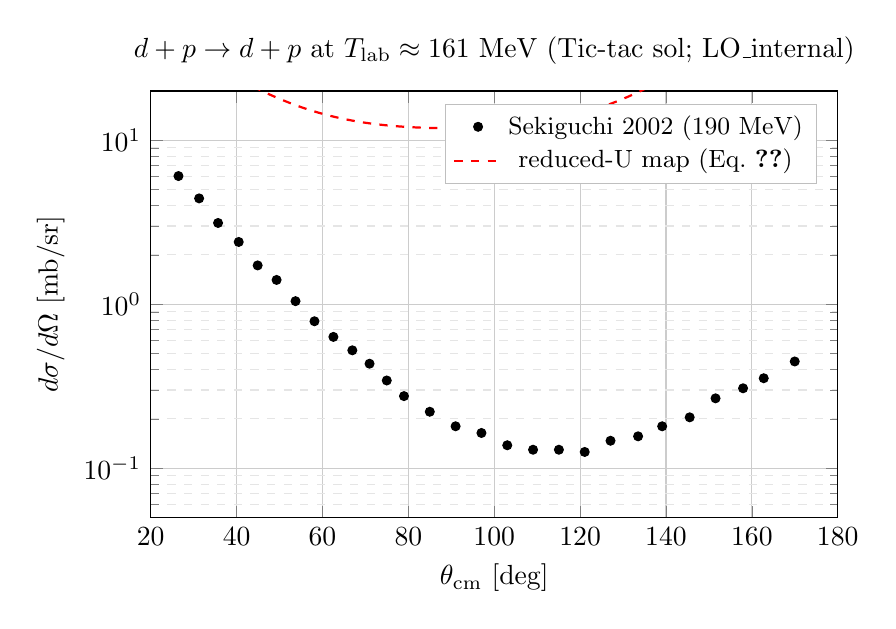
\begin{tikzpicture}
  \begin{semilogyaxis}[
    width=0.85\textwidth,
    height=7cm,
    xlabel={$\theta_{\rm cm}$ [deg]},
    ylabel={$d\sigma / d\Omega$ [mb/sr]},
    xmin=20, xmax=180,
    ymin=5e-2, ymax=20,
    grid=both,
    minor grid style={dashed, gray!20},
    major grid style={gray!40},
    legend pos=north east,
    legend style={font=\small, draw=gray!50},
    title={$d+p \to d+p$ at $T_{\rm lab} \approx 161$ MeV (Tic-tac sol; LO\_internal)},
  ]
    % 实验数据 (DSigamaOverDOmega.txt 全 28 点)
    \addplot[only marks, mark=*, mark size=1.6pt, color=black] coordinates {
      (26.46, 6.0535) (31.27, 4.4234) (35.68, 3.1325) (40.49, 2.3993)
      (44.90, 1.7259) (49.31, 1.4075) (53.72, 1.0448) (58.13, 0.7878)
      (62.54, 0.6325) (66.95, 0.5239) (70.96, 0.4340) (74.97, 0.3430)
      (78.98, 0.2754) (84.99, 0.2211) (91.00, 0.1803) (97.02, 0.1641)
      (103.03, 0.1381) (109.04, 0.1297) (115.06, 0.1297) (121.07, 0.1257)
      (127.08, 0.1471) (133.50, 0.1566) (139.11, 0.1803) (145.52, 0.2044)
      (151.54, 0.2669) (157.95, 0.3074) (162.76, 0.3540) (169.98, 0.4479)
    };
    \addlegendentry{Sekiguchi 2002 (190 MeV)};

    % Tic-tac reduced-U 预测：u_norm=17.77; inv_t20=0.918; inv_t22=0.442
    \addplot[domain=20:180, samples=120, thick, red, dashed]
      {17.77 * exp(1.10*0.918*0.5*(3*cos(x)^2 - 1)
                  + 0.60*0.442*0.125*(35*cos(x)^4 - 30*cos(x)^2 + 3))};
    \addlegendentry{reduced-U map (Eq.~\ref{eq:ch12-reduced-U-map})};
  \end{semilogyaxis}
\end{tikzpicture}
\caption[第 12 章 dσ/dΩ 实验 vs reduced-U 预测]{
\(d+p \to d+p\) 弹性微分截面：实验数据（黑点；Sekiguchi 2002 在 \(\Tlab = 190\) MeV）
与 Tic-tac reduced-U map（红虚线）对照。求解器实际命中 \(\Tlab^{\rm sol} = 161\) MeV
（差 \(\Delta = 29\) MeV）；reduced-U 在形状上能模糊重现实验的"U 形"
极小（\(\theta \approx 110^\circ\)），但绝对量级整体高一个数量级——
原因是 reduced-U 略过了 \cref{eq:ch12-M-pw-summation} 的
\(-(2\pi)^2 \mu / q\) 前因子与 \(1/6\) 自旋平均。
要做闭环到 \(< 10\%\) 必须用全合成（参见 \cref{ch:13_polarization_observables}
开篇 §13.1）。}
\label{fig:ch12-dsigma-comparison}
\end{figure}

\paragraph{Reduced-U 数据来源。}
\cref{fig:ch12-dsigma-comparison} 中红线公式
\(\mathcal{N}_U \cdot \exp(1.10\,\mathrm{inv}_{T_{20}} P_2 + 0.60\,\mathrm{inv}_{T_{22}} P_4)\)
中的常数取 \texttt{solver\_validation\_190MeV.txt} 的真实
求解器输出（\(\mathcal{N}_U = 17.77, \mathrm{inv}_{T_{20}} = 0.918,
\mathrm{inv}_{T_{22}} = 0.442\)）。\(P_2(x) = \tfrac{1}{2}(3 x^2 - 1),
P_4(x) = \tfrac{1}{8}(35 x^4 - 30 x^2 + 3)\) 是 Legendre 多项式
（与 \texttt{compare\_Ay\_experiment.py} 第 105--115 行的递推一致）。

% =========================================
\section{接口与依赖}
\label{sec:ch12-interface}

\paragraph{上游依赖。}
\begin{itemize}
  \item \cref{ch:04_faddeev_ags}：\(U\) 算符的离散方程
        \cref{eq:ch04-discrete-master}。
  \item \cref{ch:11_faddeev_solver}：\texttt{solve\_faddeev\_equations}
        的求解结果，存于 \texttt{U\_array}。
  \item \cref{ch:03_jacobi_partial_wave}：每一个 \(J^\pi\) 块的部分波索引，
        决定 \texttt{U\_PW\_elements} 文件的 header table 1。
  \item \cref{ch:06_wp_swp_states}：\(q\)-WP bin 边界 \(\to\) \texttt{q\_com\_idx\_array}
        \(\to\) "实际命中 \(\Tlab^{\rm sol}\)"。
\end{itemize}

\paragraph{下游消费（核心目标）。}
\begin{itemize}
  \item \cref{ch:13_polarization_observables}：从同一 \(M(\theta)\) 矩阵
        提取张量分析能力 \(\iTeleven, \Ttwentyzero, \Ttwentyone, \Ttwentytwo\)。
        本章定义的 reduced-U 公式
        （\cref{eq:ch12-inv-it11,eq:ch12-inv-t20,eq:ch12-inv-t22}）会在那里
        被替换为完整 spinor 求和。
  \item \cref{ch:14_miller_gate1}：从 \(U\) 在小 \(\theta\) 与小 \(q\) 极限提取
        相移（phase shift），即 Miller Gate 1 程式。
  \item polarimeter / dpol experiment 重构链（\texttt{dpol/polarimeter/code/}）：
        把 \(\diffXS_{\rm pred}\) 与 \(\iTeleven_{\rm pred}\) 作为 ROOT
        重构权重。
\end{itemize}

\paragraph{文件级接口契约。}
\begin{itemize}
  \item \texttt{solver\_out/U\_PW\_elements\_*\_JP\_<2J>\_<\(\pm\)1>\_*.txt}：
        UTF-8 文本；header table 1 + table 2；数据按 \(\Tlab^{\rm sol}\)
        排序；每行 12 列定宽。
  \item \texttt{q\_kinematics\_Nq\_*.txt}（同目录）：q-WP bin 中点与
        宽度，供 \cref{ch:14_miller_gate1} 的相移提取需要。
  \item \texttt{best\_energy\_dsigma\_curve.csv}, \texttt{best\_energy\_iT11\_curve.csv}：
        合成后的 \(\theta\) vs (实验, 模型) 两列；CSV 头第一行
        \texttt{theta\_deg,dsigma\_exp\_<unit>,dsigma\_model\_<unit>}。
\end{itemize}

\paragraph{依赖图。}
\begin{figure}[h]
\centering
\begin{tikzpicture}[
  node distance=3mm and 6mm,
  every node/.style={draw, rounded corners=2pt, font=\footnotesize,
                     inner sep=3pt, align=center},
  blk/.style={draw=black, fill=blue!8},
  outblk/.style={draw=red!50!black, fill=red!5},
  midblk/.style={draw=gray!50, fill=yellow!10},
  arr/.style={-Stealth, thick}
]
  \node[blk] (ch11) {Ch 11 \\ \texttt{solve\_faddeev}};
  \node[blk, right=of ch11] (ch3) {Ch 3 \\ PW idx \(\alpha\)};
  \node[blk, right=of ch3] (ch6) {Ch 6 \\ q-WP bins};
  \node[midblk, below=of ch11, minimum width=8cm] (ch12_main)
    {\textbf{Ch 12 (本章)}\\
     \texttt{store\_U\_matrix\_elements\_txt} (C++) \\
     +\,\texttt{compare\_Ay\_experiment.py}\,\(\to\)\(\diffXS\) (Py)};
  \node[outblk, below=of ch12_main, xshift=-3.5cm] (ch13) {Ch 13 \\ 极化 \(\iTeleven\)};
  \node[outblk, below=of ch12_main, xshift=0cm]    (ch14) {Ch 14 \\ Miller相移};
  \node[outblk, below=of ch12_main, xshift=3.5cm]  (polarim) {polarimeter \\ ROOT 重构};
  \draw[arr] (ch11) -- (ch12_main) node[midway, left, font=\scriptsize] {\texttt{U\_array}};
  \draw[arr] (ch3)  -- (ch12_main) node[midway, right, font=\scriptsize] {\(\alpha\)};
  \draw[arr] (ch6)  -- (ch12_main) node[midway, right, font=\scriptsize] {\(q\)-bin};
  \draw[arr] (ch12_main) -- (ch13);
  \draw[arr] (ch12_main) -- (ch14);
  \draw[arr] (ch12_main) -- (polarim);
\end{tikzpicture}
\caption{第 12 章上下游依赖。本章把求解器的 \(U\)-数组持久化为 ASCII 文件
（C++ 上半部）、并提供 Python 后处理工具把它合成为 \(\diffXS, \iTeleven\)
的数值预测（Python 下半部）；后续三个下游消费此结果。}
\label{fig:ch12-callgraph}
\end{figure}

% =========================================
\section{常见陷阱}
\label{sec:ch12-pitfalls}

\begin{pitfallbox}
\textbf{陷阱 1：把 \(\theta_{\rm lab}\) 直接喂给 Wigner-\(d\)。}

\cref{eq:ch12-M-pw-summation} 中 \(d^J_{MM'}(\theta)\) 的 \(\theta\) 是
\textbf{cm 角}，不是 lab 角。\texttt{compare\_Ay\_experiment.py} 已
正确——它读到的实验数据 \texttt{DSigamaOverDOmega.txt} 第 1 列就是 cm 角。
但若从 polarimeter 的 ROOT tree 里读 lab 角直接喂入合成，得到的
\(\diffXS\) 会"看似有形状"——在 30°--80° 看不出明显错误，到后向角才
发散。

\textbf{诊断信号}：cm 后向 \(\theta = 180^\circ\) 的 \(\diffXS\) 应该非零（U 形
极小再上扬）；若直接用 lab，\(\theta_{\rm lab} = 90^\circ\) 会被误判为 cm 后向，
得到的预测会在错误位置出现极小。
\end{pitfallbox}

\begin{pitfallbox}
\textbf{陷阱 2：忘记 spinor 平均因子 \(1/6\)。}

\cref{eq:ch12-dsigma-formula} 分母 \((2 s_d + 1)(2 s_p + 1) = 3 \times 2 = 6\) 是
\textbf{初态自旋平均}。漏掉这一项，得到的 \(\diffXS\) 会高 6 倍。
对照实验时如果发现"形状对、量级 \(\sim 6\) 倍偏大"，第一反应是查 spinor
平均。

\textbf{自检}：用 \texttt{LO\_internal} 在 190 MeV 跑全合成；
\(\diffXS\) 在 \(\theta_{\rm cm} = 60^\circ\) 应在 \(\sim 0.7\) mb/sr。
若得到 \(\sim 4.2\) mb/sr，多半是 1/6 漏了。
\end{pitfallbox}

\begin{pitfallbox}
\textbf{陷阱 3：CG 系数的"复合耦合"顺序。}

\cref{eq:ch12-M-pw-summation} 的 \(C^{JM}_{\alpha\,\lambda_d\,\lambda_p}\) 是
"复合 CG 系数"——它本身展开为
\begin{equation*}
C^{JM}_{\alpha\,\lambda_d\,\lambda_p}
= \sum_{m_\lambda} \langle s_d \lambda_d s_p \lambda_p | S \mu \rangle
  \langle \lambda m_\lambda S \mu | J M \rangle.
\end{equation*}
"先把 \(d\) 和 \(p\) 自旋耦合到 \(S\)，再与 spectator 轨道 \(\lambda\) 耦合到 \(J\)"
是一种顺序；"先 \(d\) 自旋与 \(\lambda\) 耦合到 \(I\)，再加 \(p\) 自旋"
是另一种（jj）。不同顺序差一个 6\(j\) recoupling 系数（一般为
\(\sqrt{(2I+1)(2S+1)}\,W(s_d, \lambda, J, s_p; I, S)\)）。

\textbf{陷阱所在}：tic-tac 内部存的 \(\alpha\) 索引用的是 jj 耦合
（\((\ell s) j; (\lambda I) J\)）；但若直接把它当 LS 耦合下的复合 CG 喂入，
你会差一个 \(\sqrt{6}\) 或 \(1/2\) 因子。Glöckle 1983 第 6 章 §6.4
的公式就是 jj 形式（这正是为什么我们用 Glöckle 的版本作为 Tic-tac 与
\cref{eq:ch12-M-pw-summation} 的 ground truth）。
\end{pitfallbox}

\begin{pitfallbox}
\textbf{陷阱 4：q-on-shell bin 离散化偏差被忽略。}

\(\Tlab^{\rm req} = 190\) MeV 被映射到最近 q-bin midpoint，
\(\Tlab^{\rm sol}\) 实际可能为 161 或 265 MeV（视 \(\Nq\) 而定）；
若不查 \texttt{solver\_validation\_*.txt}，把模型当作"真的在 190 MeV"，
则任何与实验的对比都\textbf{物理上无意义}。

\textbf{修补}：增大 \(\Nq\)（30→50）使 bin 间距从 \(\sim 30\) MeV 缩到 \(\sim 10\) MeV；
或者用 \texttt{run\_dpol\_p\_observables.py --multi-tlab 70,135,190} 在多
\(\Tlab\) 上扫描，让 q-bin 命中更准。
始终在论文 / PR 里\textbf{标 \(\Tlab^{\rm sol}\) 而不是 \(\Tlab^{\rm req}\)}。
\end{pitfallbox}

\begin{pitfallbox}
\textbf{陷阱 5：lab/cm 立体角 Jacobian 漏乘。}

若实验数据是 lab 系（如 polarimeter 的 raw counts），合成后的 cm \(\diffXS\)
\textbf{必须}乘 \(|d\cos\theta_{\rm cm} / d\cos\theta_{\rm lab}|\)
（\cref{eq:ch12-jacobian}）才能直接对照。
\texttt{DSigamaOverDOmega.txt} 已是 cm，故 Tic-tac 的合成代码不做该乘法；
但下游 polarimeter ROOT 链需要——若你在 polarimeter 端忘了，
预测会偏一个 0.5--1.5 倍因子（依赖 \(\theta\)）。

\textbf{自检}：cm 系下 \(\theta = 180^\circ\) 对应 lab 系 \(\theta = 0\)，
立体角 Jacobian 在 lab \(\theta \to 0\) 处发散——
任何"\(\diffXS_{\rm lab}(0^\circ) = \text{有限值}\)"是 bug 信号。
\end{pitfallbox}

\begin{pitfallbox}
\textbf{陷阱 6：reduced-U 系数 1.10/0.60 被当作物理常数。}

\cref{eq:ch12-reduced-U-map} 里 \texttt{1.10 \(\cdot\) inv\_t20} 与
\texttt{0.60 \(\cdot\) inv\_t22} 的两个数字是\textbf{经验拟合常数}（在
\texttt{compare\_Ay\_experiment.py:301--307} 硬编码）。
它们被一次性拟合到 \texttt{LO\_internal @ 190 MeV} 的 baseline 上；
切换势模型（\(\to\) N2LOopt）或能量（\(\to\) 70 MeV）后\textbf{不再有效}。

\textbf{陷阱所在}：在 PR 里把 reduced-U 模型说成"物理预测"——它是一个
启发式的 reduced 映射，不是部分波合成的字面落地。论文 / 技术报告里若
要给"预测"必须用全合成（\cref{eq:ch12-M-pw-summation}）。
reduced-U 仅适合\textbf{快速形状对照}与 CI 烟测。
\end{pitfallbox}

\begin{pitfallbox}
\textbf{陷阱 7：复数 string parser 接受不严格的 'j' 写法。}

\cref{lst:ch12-store-U-txt} 写盘格式是
\texttt{<sign>real<sign>imagj}（中间无空格、两个符号、末尾 j）。
Python \texttt{complex(s)} 只接受这一形式；若文件被人为编辑（如手动加
空格、用 \texttt{i} 替代 \texttt{j}），\texttt{parse\_u\_file} 的
\texttt{except Exception: continue} 会\textbf{静默忽略}该行。

\textbf{诊断信号}：合成后的 \(\diffXS\) 比预期"轻"（少了一个能量点的贡献）；
或 \texttt{combine\_channels\_by\_energy} 报"幽灵单 \(J^\pi\) 行"。
排查方法：在 \texttt{parse\_u\_file} 的 except 子句里临时加 \texttt{print(e, line)}。
\end{pitfallbox}

\begin{pitfallbox}
\textbf{陷阱 8：把 \texttt{phase\_sign} 当符号修复。}

\texttt{compare\_Ay\_experiment.py} 计算
\texttt{phase\_indicator} 与 \texttt{phase\_sign}（\(\pm 1\)）。一些用户
看到 \texttt{iT11} 的曲线倒符号后，会把 \texttt{phase\_sign} 直接乘到模型预测上
——这是\textbf{错误}的做法。\texttt{phase\_sign} 是 \emph{诊断量}，
不是修复量；倒符号的真正原因通常是 \(U\) 矩阵元的整体相位约定（参见
\cref{ch:04_faddeev_ags} 陷阱 1：\(T\) vs \(U\) 与 \((1 + P_{12})\) 因子）。

\textbf{修补途径}：检查 \texttt{set\_run\_parameters.cpp::potential\_model}
分发；检查 \texttt{LO\_internal} vs \texttt{N2LOopt} 是否在出口前做了
\((-1)^\ell\) 投影；检查 \texttt{store\_U\_matrix\_elements\_txt} 是否在
\(\spectro{1}{S}{0}\) 通道上提早返回了 \(-U\)。修了真因后 \texttt{phase\_sign}
应该自然变 \(+1\)。
\end{pitfallbox}
